\section{Static Pattern classification on Real World Data}

\subsection{MLFFNN with 2 hidden layers}
 
 The given real world data is classified using Multi Layer Feed Forward Networks with 2 hidden layers. The Neural Network is built using pytorch. We experimented with the number of nodes in each hidden layer, the optimizers(ADAM \& SGD), the learning rate and the number of epochs. Cross Entropy Loss is used for all the models built since it is known to perform better for conventional classification problems. ReLu Activation layer is used for the hidden layers. Let us look at the difference performance characteristics of the models. [x y] refers to the number of nodes in the hidden layer.
 
 It was observed that as the number of nodes in hidden layer increased, the performance increases. Similarly as the number of epochs increases, the model tends to learn better. On the other hand increasing the learning rate results in poor performance and there will be so much oscillations during convergence. The activation function is kept as ReLu for the hidden layers. After increasing the number of nodes, the model starts to overfit. The test accuracy is 64.66$\%$ for the best model.
% -----------------------------------------------------------
{\rowcolors{3}{green!40!yellow!10}{green!0!yellow!30}
\begin{table}[!h]
\centering
\begin{tabular}{ |c|c|c|  }
\hline
\rowcolor{lightgray} Model & Training Accuracy & Val Accuracy\\
\hline
[40 20]/lr=0.001/epoch=30 & 40.38$\%$  & 54.16$\%$  \\ 
\hline
[80 40]/lr=0.001/epoch=30 & 39.67$\%$  & 53.125$\%$  \\ 
\hline
[80 40]/lr=0.01/epoch=30 & 22.67$\%$  & 14.10$\%$  \\ 
\hline
[120 80]/lr=0.001/epoch=30 & 45.19$\%$  & 49.75$\%$  \\ 
\hline
[240 160]/lr=0.001/epoch=30 & 50.40$\%$  & 48.72$\%$  \\ 
\hline
[500 250]/lr=0.001/epoch=30 & 51.28$\%$  & 50$\%$  \\ 
\hline
[500 250]/lr=0.001/epoch=500 & 95.19$\%$  & 57.65$\%$  \\ 
\hline
[500 250]/lr=0.001/epoch=700 & 98.23$\%$  & 52.33$\%$  \\ 
\hline
[500 500]/lr=0.001/epoch=500 & 92.94$\%$  & 53.16$\%$  \\ 
\hline
\end{tabular}
\caption{Performance of various MLFFNN Models}.
\label{table:3}
\end{table}
}

%---------------------------------------------------------

\begin{figure}[!ht]
    \centering
    \begin{subfigure}[t]{0.5\textwidth}
        \centering
        \includegraphics[height=2.5in]{Dataset_2a/dataset_2a_cmatrix_train_data_mlffnn.png}
        \caption{Confusion Matrix for training data}
    \end{subfigure}%
    ~ 
    \begin{subfigure}[t]{0.5\textwidth}
        \centering
        \includegraphics[height=2.5in]{Dataset_2a/dataset_2a_cmatrix_test_data_mlffnn.png}/
        \caption{Confusion Matrix for test data}
    \end{subfigure}%
    ~
    \caption{Confusion Matrix for the best model}
    \label{fig:13}
\end{figure}

%-----------------------------------------------------------
\newpage
\subsection{SVM with Gaussian Kernel}
The given real world data is classified using Support Vector Classifier with One Vs the Rest Approach. Sklearn was used to implement the method. It was tried with gaussian kernels. Let us look at the performance of the various models by changing different parameters. 


For the SVM Model with gaussian kernel we experimented with the regularization parameter since there were not much to experiment with. As the value of C increases, we see that the training accuracy and validation increases. However it doesn't seem to affect the validation accuracy much. The parameter C takes care of regularization and it is inversely proportional to the strength of regularization. The best model test accuracy is 56.11$\%$

% -----------------------------------------------------------
{\rowcolors{3}{green!40!yellow!10}{green!0!yellow!30}
\begin{table}[!h]
\centering
\begin{tabular}{ |c|c|c|  }
\hline
\rowcolor{lightgray} Model & Training Accuracy & Val Accuracy\\
\hline
C=1 & 78.24$\%$  & 55$\%$  \\ 
\hline
C=3 & 85.47$\%$  & 57.78$\%$  \\ 
\hline
C=6 & 90.01$\%$  & 57.22$\%$  \\ 
\hline
C=10 & 93.26$\%$  & 53.33$\%$  \\ 
\hline
C=15 & 95.29$\%$  & 56.11$\%$  \\ 
\hline
\end{tabular}
\caption{Performance of various SVM Models with gaussian kernels}.
\label{table:3}
\end{table}
}

%---------------------------------------------------------

\begin{figure}[!ht]
    \centering
    \begin{subfigure}[t]{0.5\textwidth}
        \centering
        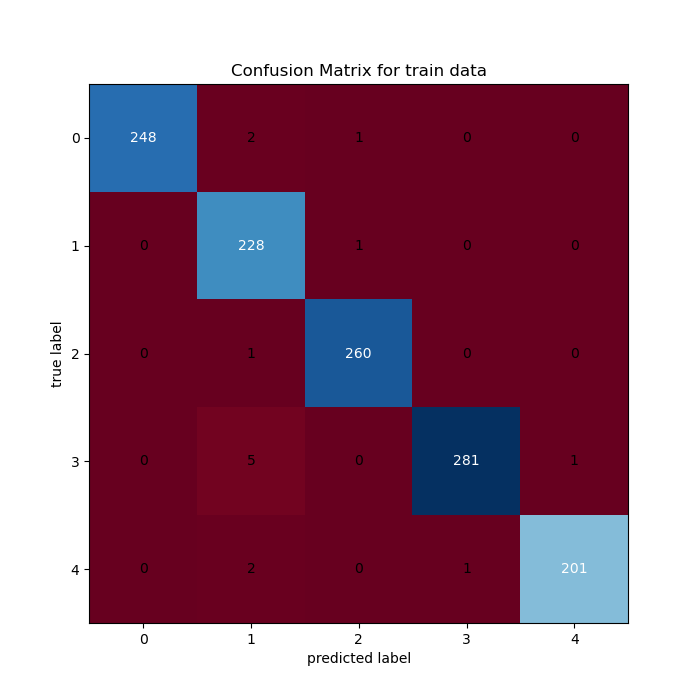
\includegraphics[height=2.5in]{Dataset_2a/dataset_2a_cmatrix_train_data_svc.png}
        \caption{Confusion Matrix for training data}
    \end{subfigure}%
    ~ 
    \begin{subfigure}[t]{0.5\textwidth}
        \centering
        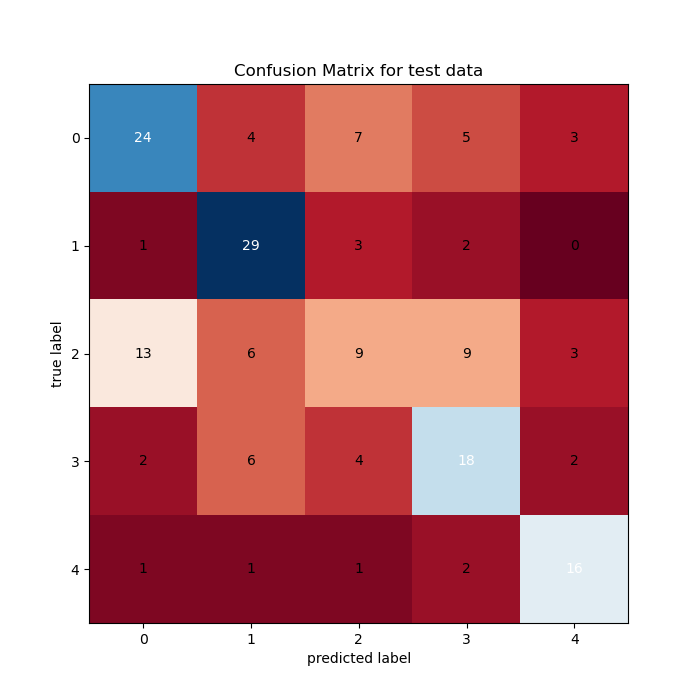
\includegraphics[height=2.5in]{Dataset_2a/dataset_2a_cmatrix_test_data_svc.png}
        \caption{Confusion Matrix for test data}
    \end{subfigure}%
    ~
    \caption{Confusion Matrix for the best model}
    \label{fig:13}
\end{figure}

%---------------------------------------------------------